% !Mode:: "TeX:UTF-8"

\def\usewhat{pdflatex}                               % 定义编译方式 dvipdfmx 或者 pdflatex,默认为 dvipdfmx
                                                     % 方式编译,如果需要修改,只需改变花括号中的内容即可。
\documentclass[12pt,openany,oneside,ctexartutf8]{book}
                                                     % 本科生毕业论文通常采用单页排版
% !Mode:: "TeX:UTF-8"
%  Authors: 张井   Jing Zhang: prayever@gmail.com     天津大学2010级管理与经济学部信息管理与信息系统专业硕士生
%           余蓝涛 Lantao Yu: lantaoyu1991@gmail.com  天津大学2008级精密仪器与光电子工程学院测控技术与仪器专业本科生

%%%%%%%%%% Package %%%%%%%%%%%%
\usepackage{graphicx}                       % 支持插图处理
% \usepackage[a4paper,text={146.4true mm,239.2 true mm},top= 25.4true mm, bottom= 25.4true mm, left=31.7 true mm,head=6true mm,headsep=6.5true mm,foot=16.5true mm]{geometry}
\usepackage[a4paper,top=25.4mm, bottom=25.4mm, left=31.7mm, right=31.7mm, head=6true mm,headsep=6.5true mm,foot=17.5mm]{geometry}
                                            % 支持版面尺寸设置
\usepackage[squaren]{SIunits}               % 支持国际标准单位


\usepackage{float}
\usepackage[table,xcdraw]{xcolor}
% \usepackage{subcaption}



\usepackage{titlesec}                       % 控制标题的宏包
\usepackage{titletoc}                       % 控制目录的宏包
\usepackage{fancyhdr}                       % fancyhdr宏包 支持页眉和页脚的相关定义
\usepackage[UTF8]{ctex}                     % 支持中文显示
\usepackage{CJKpunct}
\usepackage{color}                          % 支持彩色
\usepackage{amsmath}                        % AMSLaTeX宏包 用来排出更加漂亮的公式
\usepackage{amssymb}                        % 数学符号生成命令
\usepackage[below]{placeins}    %允许上一个section的浮动图形出现在下一个section的开始部分,还提供\FloatBarrier命令,使所有未处理的浮动图形立即被处理
\usepackage{multirow}                       % 使用Multirow宏包,使得表格可以合并多个row格
\usepackage{booktabs}                       % 表格,横的粗线;\specialrule{1pt}{0pt}{0pt}
\usepackage{longtable}                      % 支持跨页的表格。
\usepackage{tabularx}                       % 自动设置表格的列宽
\usepackage{subfigure}                      % 支持子图 %centerlast 设置最后一行是否居中
\usepackage[subfigure]{ccaption}            % 支持子图的中文标题
\usepackage[sort&compress,numbers]{natbib}  % 支持引用缩写的宏包
\usepackage{enumitem}                       % 使用enumitem宏包,改变列表项的格式
\usepackage{calc}                           % 长度可以用+ - * / 进行计算
\usepackage{txfonts}                        % 字体宏包
\usepackage{bm}                             % 处理数学公式中的黑斜体的宏包
\usepackage[amsmath,thmmarks,hyperref]{ntheorem}  % 定理类环境宏包,其中 amsmath 选项用来兼容 AMS LaTeX 的宏包
\usepackage{CJKnumb}                        % 提供将阿拉伯数字转换成中文数字的命令
\usepackage{indentfirst}                    % 首行缩进宏包
% \usepackage{CJKutf8}                        % 用在UTF8编码环境下,它可以自动调用CJK,同时针对UTF8编码作了设置

% \usepackage{fancybox} 

%\usepackage{hypbmsec}                      % 用来控制书签中标题显示内容
\newcommand{\tabincell}[2]{\begin{tabular}{@{}#1@{}}#2\end{tabular}}
\usepackage{xcolor}
%支持代码环境
\usepackage{listings}
\lstset{numbers=left,
language=[ANSI]{C},
numberstyle=\tiny,
extendedchars=false,
showstringspaces=false,
breakatwhitespace=false,
breaklines=true,
captionpos=b,
keywordstyle=\color{blue!70},
commentstyle=\color{red!50!green!50!blue!50},
frame=shadowbox,
rulesepcolor=\color{red!20!green!20!blue!20}
}
%支持算法环境
\usepackage[boxed,ruled,lined]{algorithm2e}
\usepackage{algorithmic}

\usepackage{array}
\newcommand{\PreserveBackslash}[1]{\let\temp=\\#1\let\\=\temp}
\newcolumntype{C}[1]{>{\PreserveBackslash\centering}p{#1}}
\newcolumntype{R}[1]{>{\PreserveBackslash\raggedleft}p{#1}}
\newcolumntype{L}[1]{>{\PreserveBackslash\raggedright}p{#1}}

% 生成有书签的 pdf 及其生成方式。通常可以在 tjumain.tex 文件的第一行选择 pdflatex 或者是 dvipdfmx 编译手段。如果选择前者,则使用 pdflatex + pdflatex 编译; 如果选择后者,在编译的时候选择 latex + bibtex + latex + latex 编译。出现混淆的时候,系统会报错。
% 如果您的pdf制作中文书签有乱码使用如下命令,就可以解决了
\def\atemp{pdflatex}\ifx\atemp\usewhat
\usepackage{cmap}                           % pdflatex 编译时,可以生成可复制、粘贴的中文 PDF 文档, 缺点是在Windows上显示时效果不大好,字体发虚
\usepackage{hyperref}
\hypersetup{
    unicode,
    pdfborder={0 0 0},
}
\fi
% \usepackage[pdftex,unicode,
%             CJKbookmarks=true,
%             bookmarksnumbered=true,
%             bookmarksopen=true,
%             colorlinks=false,
%             pdfborder={0 0 0},
%             citecolor=blue,
%             linkcolor=red,
%             anchorcolor=green,
%             urlcolor=blue,
%             breaklinks=true
%             ]{hyperref}

                                % 定义本文所使用宏包
\graphicspath{{figures/}}                            % 定义所有的 .eps 文件在 figures 子目录下


\begin{document}                                     % 开始全文
	% !Mode:: "TeX:UTF-8"
%  Authors: 张井   Jing Zhang: prayever@gmail.com     天津大学2010级管理与经济学部信息管理与信息系统专业硕士生
%           余蓝涛 Lantao Yu: lantaoyu1991@gmail.com  天津大学2008级精密仪器与光电子工程学院测控技术与仪器专业本科生

% 2018/5/23修正
%           李幼萌 Youmeng Li: liyoumeng@tju.edu.cn   天津大学软件学院软件工程系

%%%%%%%%%%%%%%%%% Fonts Definition and Basics %%%%%%%%%%%%%%%%%
\newcommand{\song}{\CJKfamily{song}}    % 宋体
\newcommand{\fs}{\CJKfamily{fs}}        % 仿宋体
\newcommand{\kai}{\CJKfamily{kai}}      % 楷体
\newcommand{\hei}{\CJKfamily{hei}}      % 黑体
\newcommand{\li}{\CJKfamily{li}}        % 隶书
\newcommand{\yihao}{\fontsize{26pt}{26pt}\selectfont}       % 一号, 单倍行距
\newcommand{\xiaoyi}{\fontsize{24pt}{24pt}\selectfont}      % 小一, 单倍行距
\newcommand{\erhao}{\fontsize{22pt}{1.25\baselineskip}\selectfont}       % 二号, 1.25倍行距
\newcommand{\xiaoer}{\fontsize{18pt}{18pt}\selectfont}      % 小二, 单倍行距
\newcommand{\sanhao}{\fontsize{16pt}{16pt}\selectfont}      % 三号, 单倍行距
\newcommand{\xiaosan}{\fontsize{15pt}{15pt}\selectfont}     % 小三, 单倍行距
\newcommand{\sihao}{\fontsize{14pt}{14pt}\selectfont}       % 四号, 单倍行距
\newcommand{\xiaosi}{\fontsize{12pt}{12pt}\selectfont}      % 小四, 单倍行距
\newcommand{\wuhao}{\fontsize{10.5pt}{10.5pt}\selectfont}   % 五号, 单倍行距
\newcommand{\xiaowu}{\fontsize{9pt}{9pt}\selectfont}        % 小五, 单倍行距

\def\CJKtilde{\~{}}  % 简单地重新定义波浪符

\newcommand\prechaptername{第}
\newcommand\postchaptername{章}

\punctstyle{hangmobanjiao}             % 调整中文字符的表示,行内占一个字符宽度,行尾占半个字符宽度

% 调整罗列环境的布局
\setitemize{leftmargin=3em,itemsep=0em,partopsep=0em,parsep=0em,topsep=-0em}
\setenumerate{leftmargin=3em,itemsep=0em,partopsep=0em,parsep=0em,topsep=0em}

% 避免宏包 hyperref 和 arydshln 不兼容带来的目录链接失效的问题。
\def\temp{\relax}
\let\temp\addcontentsline
\gdef\addcontentsline{\phantomsection\temp}

% 自定义项目列表标签及格式 \begin{publist} 列表项 \end{publist}
\newcounter{pubctr} %自定义新计数器
\newenvironment{publist}{%%%%%定义新环境
\begin{list}{[\arabic{pubctr}]} %%标签格式
    {
     \usecounter{pubctr}
     \setlength{\leftmargin}{2.5em}   % 左边界 \leftmargin =\itemindent + \labelwidth + \labelsep
     \setlength{\itemindent}{0em}     % 标号缩进量
     \setlength{\labelsep}{1em}       % 标号和列表项之间的距离,默认0.5em
     \setlength{\rightmargin}{0em}    % 右边界
     \setlength{\topsep}{0ex}         % 列表到上下文的垂直距离
     \setlength{\parsep}{0ex}         % 段落间距
     \setlength{\itemsep}{0ex}        % 标签间距
     \setlength{\listparindent}{0pt}  % 段落缩进量
    }}
{\end{list}}

\makeatletter
\renewcommand\normalsize{
  \@setfontsize\normalsize{12pt}{12pt} % 小四对应 12 pt
  \setlength\abovedisplayskip{4pt}
  \setlength\abovedisplayshortskip{4pt}
  \setlength\belowdisplayskip{\abovedisplayskip}
  \setlength\belowdisplayshortskip{\abovedisplayshortskip}
  \let\@listi\@listI}
\def\defaultfont{\renewcommand{\baselinestretch}{1.63}\normalsize\selectfont} % 设置行距

\renewcommand{\CJKglue}{\hskip -0.1 pt plus 0.08\baselineskip} % 控制字间距,使每行 34 个汉字
\makeatother

%%%%%%%%%%%%% Contents %%%%%%%%%%%%%%%%%
\renewcommand{\contentsname}{目\qquad 录}
\setcounter{tocdepth}{1} % 控制目录深度
\titlecontents{chapter}[2em]{\vspace{.5\baselineskip}\xiaosan\song}
             {\prechaptername\CJKnumber{\thecontentslabel}\postchaptername\qquad}{}
             {\hspace{.5em}\titlerule*[10pt]{$\cdot$}\sihao\contentspage}
\titlecontents{section}[4.2em]{\vspace{.25\baselineskip}\sihao\song}
             {\thecontentslabel\quad}{}
             {\hspace{.5em}\titlerule*[10pt]{$\cdot$}\sihao\contentspage}
% \titlecontents{subsection}[4em]{\vspace{.25\baselineskip}\xiaosi\song}
%              {\thecontentslabel\quad}{}
%              {\hspace{.5em}\titlerule*[10pt]{$\cdot$}\sihao\contentspage}

%%%%%%%%%% Chapter and Section %%%%%%%%%%%%%
\setcounter{secnumdepth}{4}
\setlength{\parindent}{2em}

\renewcommand{\chaptername}{\prechaptername\CJKnumber{\thechapter}\postchaptername}
\titleformat{\chapter}{\centering}{\xiaosan\song}{\chaptername}{} %{2em}
\titlespacing{\chapter}{0pt}{0.1\baselineskip}{0.8\baselineskip}

\titleformat{\section}{\sihao\hei}{\thesection}{1em}{}
\titlespacing{\section}{0pt}{0.15\baselineskip}{0.25\baselineskip}

\titleformat{\subsection}{\sihao\hei}{\thesubsection}{1em}{}
\titlespacing{\subsection}{0pt}{0.1\baselineskip}{0.3\baselineskip}

\titleformat{\subsubsection}{\sihao\hei}{\thesubsubsection}{1em}{}
\titlespacing{\subsubsection}{0pt}{0.05\baselineskip}{0.1\baselineskip}

%%%%%%%%%% Table, Figure and Equation %%%%%%%%%%%%%%%%%
\renewcommand{\tablename}{表}                                     % 插表题头
\renewcommand{\figurename}{图}                                    % 插图题头
\renewcommand{\thefigure}{\arabic{chapter}-\arabic{figure}}       % 使图编号为 7-1 的格式 %\protect{~}
\renewcommand{\thesubfigure}{\alph{subfigure})}                   % 使子图编号为 a) 的格式
\renewcommand{\thesubtable}{(\alph{subtable})}                    % 使子表编号为 (a) 的格式
\renewcommand{\thetable}{\arabic{chapter}-\arabic{table}}         % 使表编号为 7-1 的格式
\renewcommand{\theequation}{\arabic{chapter}-\arabic{equation}}   % 使公式编号为 7-1 的格式

%%%%%% 定制浮动图形和表格标题样式 %%%%%%
\makeatletter
\long\def\@makecaption#1#2{
   \vskip\abovecaptionskip
   \sbox\@tempboxa{\centering\wuhao\song{#1\qquad #2} }
   \ifdim \wd\@tempboxa >\hsize
     \centering\wuhao\song{#1\qquad #2} \par
   \else
     \global \@minipagefalse
     \hb@xt@\hsize{\hfil\box\@tempboxa\hfil}
   \fi
   \vskip\belowcaptionskip}
\makeatother
\captiondelim{~~~~} %用来控制longtable表头分隔符

%%%%%%%%%% Theorem Environment %%%%%%%%%%%%%%%%%
\theoremstyle{plain}
\theorembodyfont{\song\rmfamily}
\theoremheaderfont{\hei\rmfamily}
\newtheorem{theorem}{定理~}[chapter]
\newtheorem{lemma}{引理~}[chapter]
\newtheorem{axiom}{公理~}[chapter]
\newtheorem{proposition}{命题~}[chapter]
\newtheorem{prop}{性质~}[chapter]
\newtheorem{corollary}{推论~}[chapter]
\newtheorem{definition}{定义~}[chapter]
\newtheorem{conjecture}{猜想~}[chapter]
\newtheorem{example}{例~}[chapter]
\newtheorem{remark}{注~}[chapter]
%\newtheorem{algorithm}{算法~}[chapter]
\newenvironment{proof}{\noindent{\hei 证明:}}{\hfill $ \square $ \vskip 4mm}
\theoremsymbol{$\square$}

%%%%%%%%%% Page: number, header and footer  %%%%%%%%%%%%%%%%%

%\frontmatter 或 \pagenumbering{roman}
%\mainmatter 或 \pagenumbering{arabic}
\makeatletter
\renewcommand\frontmatter{\clearpage
  \@mainmatterfalse
  }
\makeatother

%%%%%%%%%%%% References %%%%%%%%%%%%%%%%%
\renewcommand{\bibname}{参考文献}
% 重定义参考文献样式,来自thu
\makeatletter
\renewenvironment{thebibliography}[1]{
    \titleformat{\chapter}{\raggedright\sihao\hei}{\chaptername}{2em}{}
   \chapter*{\bibname}
   \wuhao
   \list{\@biblabel{\@arabic\c@enumiv}}
        {\renewcommand{\makelabel}[1]{##1\hfill}
         \settowidth\labelwidth{0 cm}
         \setlength{\labelsep}{0pt}
         \setlength{\itemindent}{0pt}
         \setlength{\leftmargin}{\labelwidth+\labelsep}
         \addtolength{\itemsep}{-0.7em}
         \usecounter{enumiv}
         \let\p@enumiv\@empty
         \renewcommand\theenumiv{\@arabic\c@enumiv}}
    \sloppy\frenchspacing
    \clubpenalty4000
    \@clubpenalty \clubpenalty
    \widowpenalty4000
    \interlinepenalty4000
    \sfcode`\.\@m}
   {\def\@noitemerr
     {\@latex@warning{Empty `thebibliography' environment}}
    \endlist\frenchspacing}
\makeatother

\addtolength{\bibsep}{-0.5em}     % 缩小参考文献间的垂直间距
\setlength{\bibhang}{2em}         % 每个条目自第二行起缩进的距离

% 参考文献引用作为上标出现
%\newcommand{\citeup}[1]{\textsuperscript{\cite{#1}}}
\makeatletter
    \def\@cite#1#2{\textsuperscript{[{#1\if@tempswa , #2\fi}]}}
\makeatother
%% 引用格式
\bibpunct{[}{]}{,}{s}{}{,}

%%%%%%%%%%%% Cover %%%%%%%%%%%%%%%%%
% 封面、摘要、版权、致谢格式定义
\makeatletter
\def\ctitle#1{\def\@ctitle{#1}}\def\@ctitle{}
\def\cdegree#1{\def\@cdegree{#1}}\def\@cdegree{}
\def\caffil#1{\def\@caffil{#1}}\def\@caffil{}
\def\csubject#1{\def\@csubject{#1}}\def\@csubject{}
\def\cgrade#1{\def\@cgrade{#1}}\def\@cgrade{}
\def\cauthor#1{\def\@cauthor{#1}}\def\@cauthor{}
\def\cnumber#1{\def\@cnumber{#1}}\def\@cnumber{}
\def\cstuid#1{\def\@cstuid{#1}}\def\@cstuid{}
\def\cdate#1{\def\@cdate{#1}}\def\@cdate{}
\long\def\cabstract#1{\long\def\@cabstract{#1}}\long\def\@cabstract{}
\long\def\eabstract#1{\long\def\@eabstract{#1}}\long\def\@eabstract{}
\def\ckeywords#1{\def\@ckeywords{#1}}\def\@ckeywords{}
\def\ekeywords#1{\def\@ekeywords{#1}}\def\@ekeywords{}
\def\cheading#1{\def\@cheading{#1}}\def\@cheading{}
\def\ccovertitle#1{\def\@ccovertitle{#1}}\def\@ccovertitle{}

\pagestyle{fancy}
  \fancyhf{}
  \fancyhead[C]{\song\wuhao \@cheading}  % 页眉显示天津大学 20XX 届本科生毕业论文
  \fancyfoot[C]{\song\xiaowu ~\thepage~}
\newlength{\@title@width}

% 定义封面
\def\makecover{
%\cleardoublepage%
   \phantomsection
    \pdfbookmark[-1]{\@ctitle}{ctitle}

    \begin{titlepage}
      \vspace*{10pt}
      \begin{center}

      \begin{figure}[h]
      \centering
      
\includegraphics[width=0.4\textwidth]{figures/tju}
      \end{figure}
      \vspace*{15pt}
      \hei\erhao{\textbf{\@ccovertitle}} \\
      \hei\erhao{\textbf{\@ctitle}}
      \vspace*{55pt}

      \begin{figure}[h]
      \centering
      
\includegraphics[width=0.3\textwidth]{figures/Tjulogo}
      \end{figure}

      \vspace*{60pt}
      \renewcommand\arraystretch{1.5}
      \setlength{\@title@width}{5cm}
      {
        \sanhao\song{
          \begin{tabular}{lc}
            \textbf{学\qquad 院}  &  \underline{\makebox[\@title@width][c]{\textbf{\@caffil}}} \\
            \textbf{专\qquad 业}  &  \underline{\makebox[\@title@width][c]{\textbf{\@csubject}}} \\
            \textbf{年\qquad 级}  &  \underline{\makebox[\@title@width][c]{\textbf{\@cgrade}}}\\
            \textbf{姓\qquad 名}  &  \underline{\makebox[\@title@width][c]{\textbf{\@cauthor}}}\\
            \textbf{学\qquad 号}  &  \underline{\makebox[\@title@width][c]{\textbf{\@cstuid}}}\\
          \end{tabular}
        }
    }
    \vspace*{40pt}

    \song\sanhao{\textbf{\@cdate}}
    \end{center}
    \end{titlepage}
}

                             % 完成对论文各个部分格式的设置
	% !Mode:: "TeX:UTF-8"


%%%%%%%%%%%%%%%%%%%%%%%%%%%%%%%%%%%%%%%%%%%%%%%%%%%%%%%%%%%%%%%
%%  可通过对 setup/format.tex中                               %%
%%  第243行 \setlength{\@title@width}{5cm}中 5cm 这个参数来   %%
%%  控制封面中下划线的长度。                                   %%
%%%%%%%%%%%%%%%%%%%%%%%%%%%%%%%%%%%%%%%%%%%%%%%%%%%%%%%%%%%%%%

\cheading{天津大学软件工程~\the\year~年《软件工程综合实践》结课报告}      % 正文页眉
\ccovertitle{《软件工程综合实践》结课报告}                       % 封面标题

%%%%%%%%%%%%%%%%%%%%%%%%%%%%%%%%%%%%%%%%%%%%%%%%%%%%%%%%%%%%%
%%%%%%%%%% 以下为论文的基本信息,需要由作者进行修改 %%%%%%%%%%%%
%%%%%%%%%%%%%%%%%%%%%%%%%%%%%%%%%%%%%%%%%%%%%%%%%%%%%%%%%%%%%
\newcommand{\cauthorTwo}[1]{\def\cauthorTwoText{#1}}
\ctitle{第51组实验报告
}    
\caffil{智能与计算学部}       % 学院名称
\csubject{软件工程}     % 专业名称
\cgrade{2022级}           % 年级
\cauthor{覃邱维~王俊哲~聂哲浩~李亮克}          % 学生姓名 
\cstuid{30222444(55~31~26~34) }     % 学号 

\cdate{2024~年~9~月~12~日}  % 论文完成日期,不需要修改,自动生成

	\frontmatter                                     % 以下是论文导言部分,包括论文的封面,中英文摘要和中文目录
	\fancypagestyle{plain}{							 % 正文前均无页眉
		\fancyhf{}
		\renewcommand{\headrulewidth}{0 pt}
		\fancyfoot[C]{\song\xiaowu~\thepage~}
	}

	\makecover 			% 封面

	% !Mode:: "TeX:UTF-8"

% 目录
\defaultfont
\clearpage{
    \pagestyle{empty}
    \cleardoublepage
    \setcounter{page}{1}                                 % 单独从 1 开始编页码
    \pagenumbering{arabic}
    \titleformat{\chapter}{\centering\sanhao\hei}{\chaptername}{2em}{} % 设置目录两字的格式
    \pdfbookmark[0]{目~~录}{mulu}
    \tableofcontents                                     % 中文目录
    \thispagestyle{plain}
} % 目录

	\mainmatter\defaultfont\sloppy\raggedbottom
	\makeatletter
	\fancypagestyle{plain}{                              % 设置正文眉页脚风格
		\fancyhf{}
		\fancyhead[C]{\song\wuhao \@cheading}            % 页眉格式
		\fancyfoot[C]{\song\xiaowu ~\thepage~}           % 页脚格式
		\renewcommand{\headrulewidth}{0.5pt}
		\renewcommand{\footrulewidth}{0pt}
	}
	\makeatother
	\setcounter{page}{1}                                 % 单独从 1 开始编页码
	\titleformat{\chapter}{\centering\xiaosan\hei}{\chaptername}{2em}{} % 恢复chapter标题格式要求

	%%%%%% 这里是正文,每个文件对应正文中的一章 %%%%%%
\chapter{软件需求规格说明书}

\section{引言}

\subsection{简介}

本文档的目的是详细地介绍 饿了吧 APP所包含的需求,以便客户能够确认产品的确切需求以及开发人员能够根据需求设计编码,以下叙述将结合文字描述、UML图、ER图等来描述 饿了吧 APP的功能、性能、用户界面、运行环境、外部接口以及针对用户操作给出的各种响应。本文档的预期读者有用户及客户、项目经理、开发人员以及跟该项目相关的其他竞争人员。

\subsection{背景}
\subsubsection{项目背景}
作为天津大学智算学部暑假到T软公司实习的学生。上班第一天,老板告诉我们,公司现在有个紧急项目,要求三周后上线,但是……上周末,这个项目唯一的程序员,小东,因不满公司的薪水待遇过低而离职了,现在留下了一个半成品的烂摊子,重担就这样落在了我们几个毫无开发经验的实习生身上……


T软公司为了站在互联网的风口起飞,决定快速开发一个互联网APP,模仿著名的互联网点外卖的APP“饿了么”,开发一个竞品APP“饿了吧”。此项目要求必须三周内上线,时间紧任务重,本着小步快跑、快速迭代的原则,“饿了吧”第一期仅开发下列功能:
\begin{itemize}
    \item 商家入驻平台,管理待售商品。
    \item 用户注册,管理个人账号和个人信息。
    \item 用户点餐,管理购物车,管理送货地址,下单支付。
    \footnotesize
    \item 注:支付界面中点击确认后,将调用支付宝等平台完成实际支付,此功能由其他组开发,本项目组不必开发,直接返回支付成功即可。
    \normalsize
\end{itemize}

\subsubsection{开发路线}
基于公司的技术基础和偏好,本项目后续开发将延用之前采用的前后端分离的技术路线。
\begin{itemize}
    \item 后端:Spring Boot
    \item 前端:VUE 3
    \item 数据库:MySQL
\end{itemize}
\subsubsection{项目现状}
\begin{itemize}
\item 唯一的程序员小东已跑路,现在项目组只有你们几个实习生。
\item 经检查,小东仅完成了用户点餐功能,包括购物车管理、送餐地址管理、下订单几个功能,其它功能并未完成,像用户、商家、商品等数据,是在数据库中直接添加的。
\item 已完成的功能中,也存在不少问题,有功能上的问题,也有设计上的问题。
\item 现有的材料,包括
\begin{itemize}
    \item 部分不规范的文档和代码
    \item 公司要求小东录制的一些技术讲座视频,可以用来企业内部学习相关技术
\end{itemize}
\end{itemize}
\subsubsection{目前项目工作内容}
\begin{itemize}
    \item 重新进行项目需求分析,达到预期目标
    \item 项目重构,解决原项目中存在的问题
\end{itemize}









 % \begin{itemize}
 %     \item \textbf{外卖需求增长:}随着城市化进程的加快和生活节奏的加速,越来越多的人选择外卖服务,尤其是在大城市,外卖已经成为人们日常生活中不可或缺的一部分。
 %     \item \textbf{餐饮行业的数字化转型:}传统餐饮行业面临转型升级的压力,许多餐厅需要通过线上渠道来扩大顾客群并提升销售额。
 %     \item \textbf{ 消费者行为的改变:}年轻一代更倾向于通过移动互联网进行餐饮消费,他们希望在方便快捷的同时拥有更多的选择。
 % \end{itemize}



 % \begin{itemize}
 %     \item \textbf{移动互联网的发展:}智能手机的普及和移动互联网技术的发展为在线外卖平台的出现提供了技术基础。用户可以随时随地通过手机下单。
 %     \item \textbf{定位与导航技术:}GPS和北斗等地图导航技术的成熟,使得在线外卖平台能够准确定位用户位置,提供快速的配送服务。
 %     \item \textbf{支付系统的完善:}电子支付的普及为在线支付和快速交易提供了便捷的途径,这进一步促进了在线外卖业务的发展。
 % \end{itemize}

\subsection{ 定义、缩略语}


\begin{table}[h]
    \centering
    \begin{tabularx}{0.8\linewidth}{|l|X|}
    \hline
        \textbf{术语} & \textbf{解释}\\ \hline
        购物车 &用户在浏览商家菜单时选择的多个菜品和商品的临时集合,用户可以在下单之前将这些选定的商品放入购物车中。  \\
    \hline
    \end{tabularx}
    \caption{术语解释}
    \label{tab:sy}
\end{table}

\subsection{约束}
    前后端分离的设计方案,前后端使用符合RESTful风格的接口设计
\section{需要分析}

\subsection{目标}
饿了吧旨在为用户以及商家提供一款便捷,高效的在线外卖平台,支持用户在线快速浏览附近餐厅,下单并获得及时送餐服务,最终做到让用户享受简单且快速的订餐体验,同时提升餐厅的订单量和运营效率.具体而言,饿了吧最终会实现以下内容:
  \begin{enumerate}
      \item  实现用户与商家的注册行为.
      \item  用户和商家能够修改自身账号信息.
      \item  用户能够完成从点餐、查看购物车、修改订单地址到付款的点餐流程.
      \item  商家能够完成对自身商品的上架、下架、修改操作.
      \item  设置管理员登录,管理商家信息.
  \end{enumerate}

\subsection{涉众分析}
本系统只涉及第1.2.3,4类涉众,没有第5类涉众

\begin{table}[h]
\resizebox{\columnwidth}{!}{%
\begin{tabular}{|c|c|c|l|}
\hline
\textbf{序号} & \textbf{涉众} & \textbf{代表人物} & \multicolumn{1}{c|}{\textbf{待解决的问题/对系统的期望}}                                   \\ \hline
1 & 顾客 & 张三 & \begin{tabular}[c]{@{}l@{}}1.能注册账号\\ 2.能管理账号和个人信息\\ 3.能点餐,管理购物车、送货地址,下单支付\end{tabular} \\ \hline
2           & 商家          & 李四            & \begin{tabular}[c]{@{}l@{}}1.能注册账号\\ 2.能管理商家信息\\ 3.能上架、下架、管理待售商品\end{tabular} \\ \hline
3           & 管理员         & 王五            & 1.能管理用户数据                                                                     \\ \hline
4           & 审核员         & 赵六            & 1.审核商家上架商品                                                                    \\ \hline
5           & 配送员(骑手)     & 李七            & \begin{tabular}[c]{@{}l@{}}1.能获取订单信息\\ 2.获取商家以及用户地点进行取餐,送餐\end{tabular}       \\ \hline
\end{tabular}%
}
\caption{涉众分析表}
\label{tab:szfx}
\end{table}

\subsection{范围}
本系统不与实际支付接口对接,不提供针对配送员的业务流程

\section{业务分析}
\subsection{业务概念分析}
\subsubsection{概述}
饿了吧要管理的事情主要分为三个部分:用户注册,用户下订单,商家上架与下架商品.
\subsubsection{业务概念一览}
\begin{figure}[H]
    \centering
    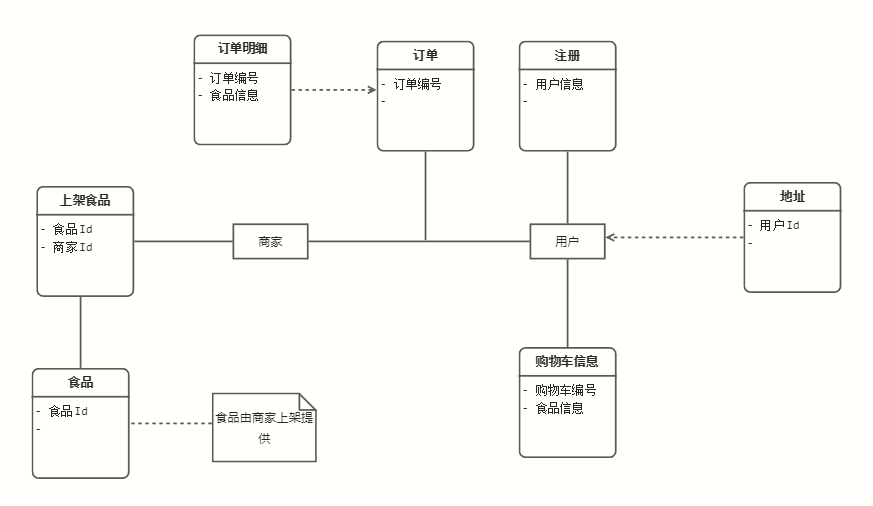
\includegraphics[width=0.90\linewidth]{pics/1.png}
    \caption{业务概念一览}
    \label{fig:ywgn}
\end{figure}

\subsubsection{登录用户}

\begin{figure}[h]
    \centering
    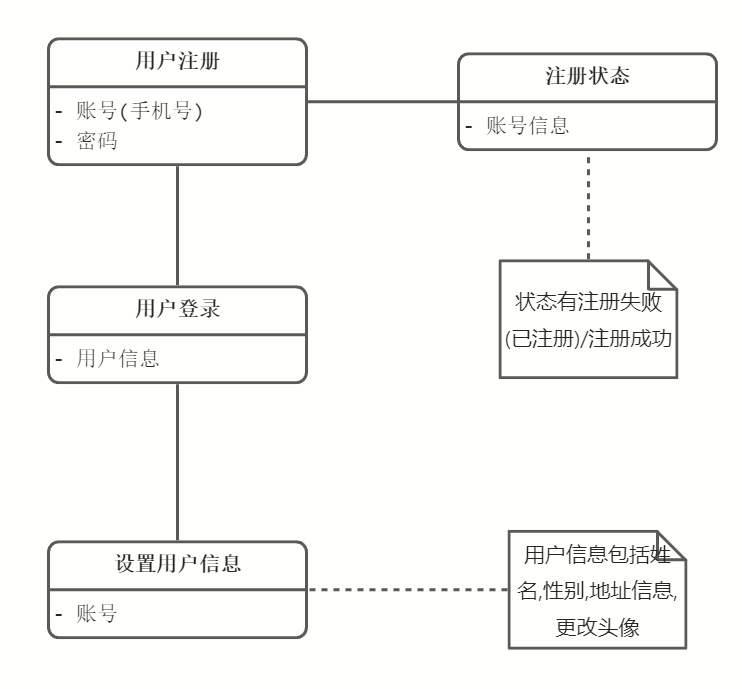
\includegraphics[width=0.5\linewidth]{pics/2.png}
    \caption{登录用户}
    \label{fig:dlyh}
\end{figure}

\subsubsection{顾客下单}
\begin{figure}[H]
    \centering
    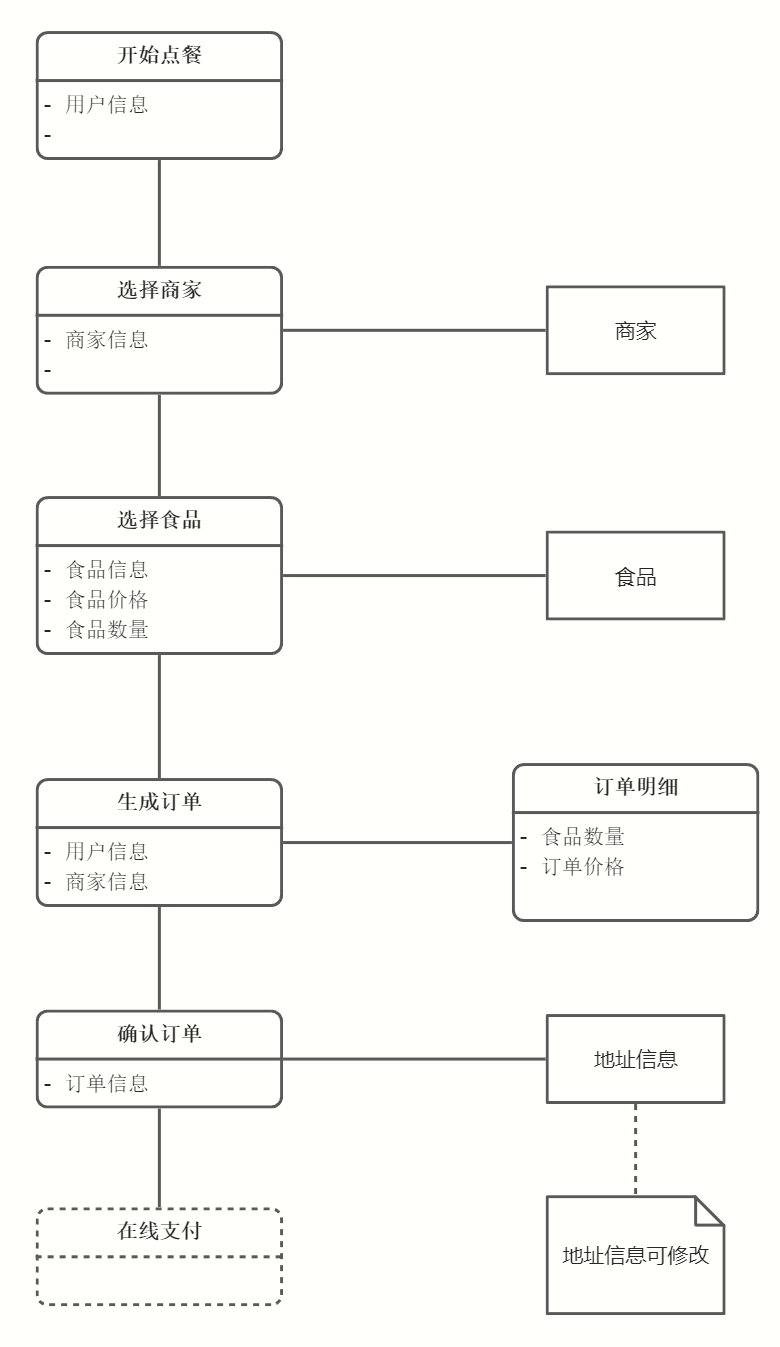
\includegraphics[width=0.7\linewidth]{pics/3.png}
    \caption{顾客下单}
    \label{fig:gkxd}
\end{figure}

\subsection{商家管理商品}

\begin{figure}[H]
    \centering
    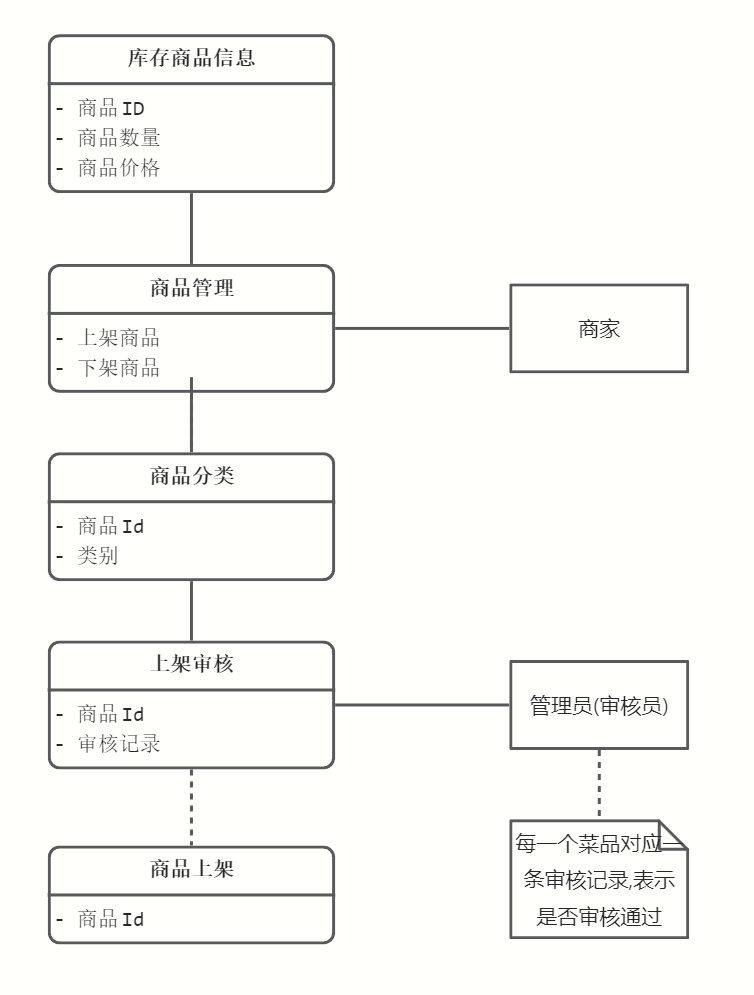
\includegraphics[width=0.4\linewidth]{pics/4.png}
    \caption{商家管理商品}
    \label{fig:sjglsp}
\end{figure}

\subsection{业务流程分析(UML活动图)}

\subsubsection{用户登录流程}

\begin{figure}[H]
    \centering
    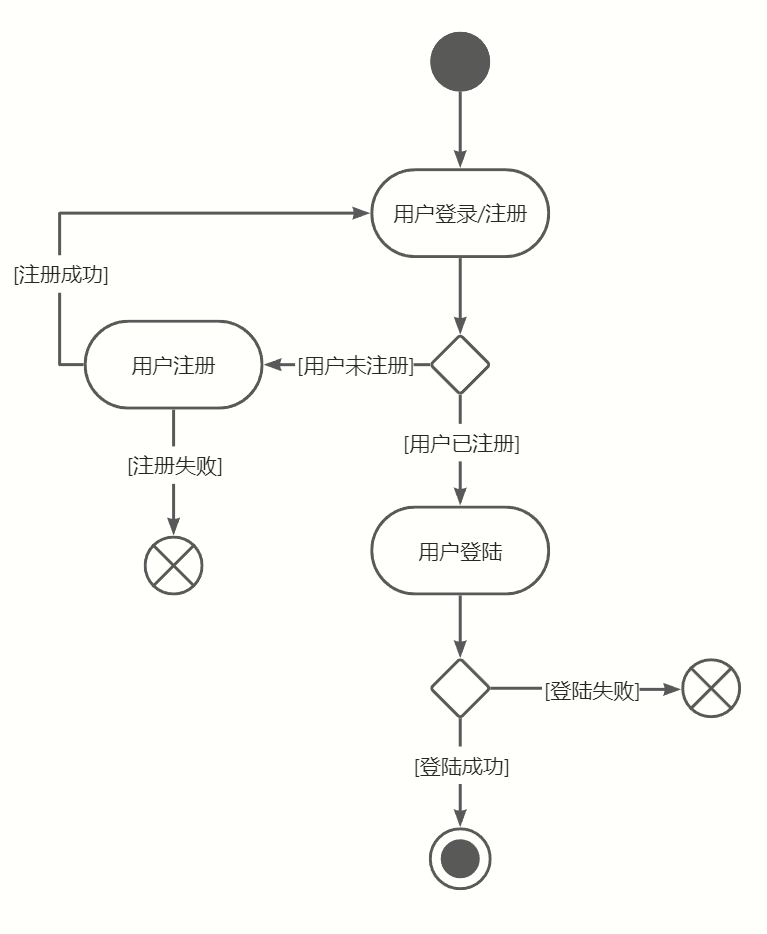
\includegraphics[width=0.5\linewidth]{pics/5.png}
    \caption{用户登录流程}
    \label{fig:yhddlc}
\end{figure}

\subsubsection{顾客下单流程}
\begin{figure}[H]
    \centering
    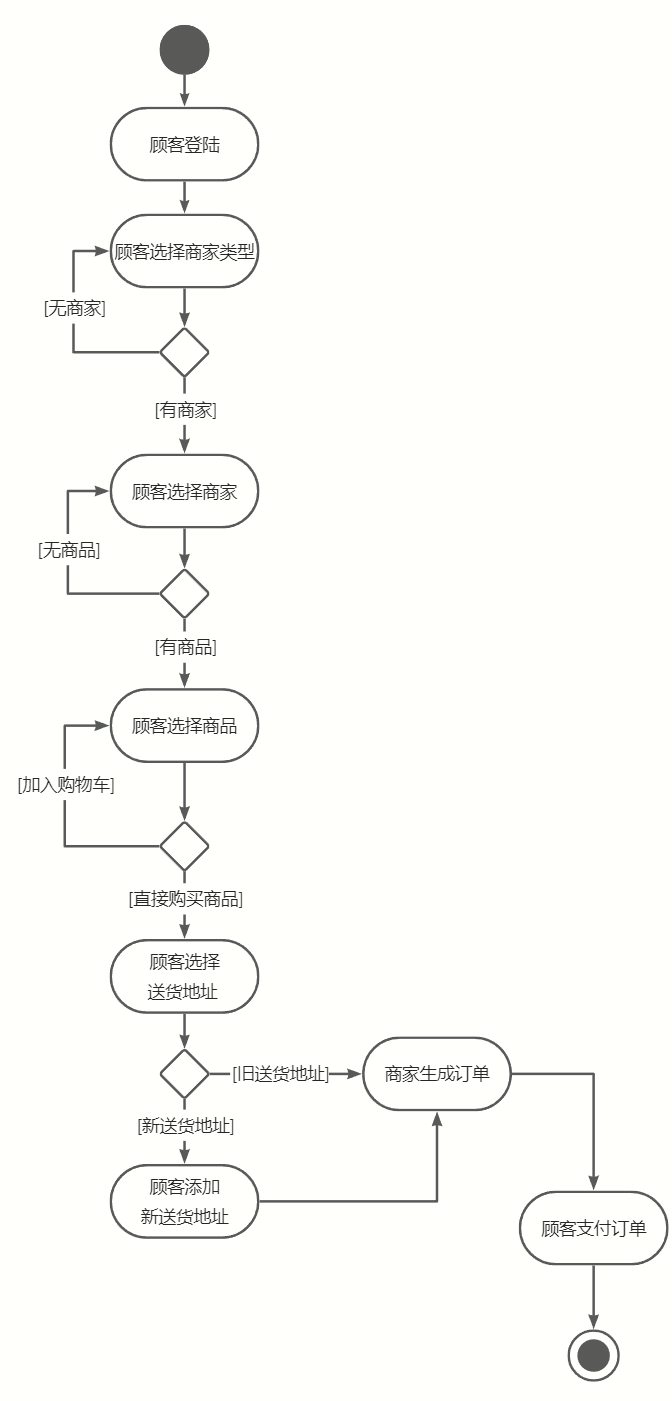
\includegraphics[width=0.5\linewidth]{pics/6.png}
    \caption{顾客下单流程}
    \label{fig:gkxdlc}
\end{figure}

\subsubsection{商家管理商品流程}
\begin{figure}[H]
    \centering
    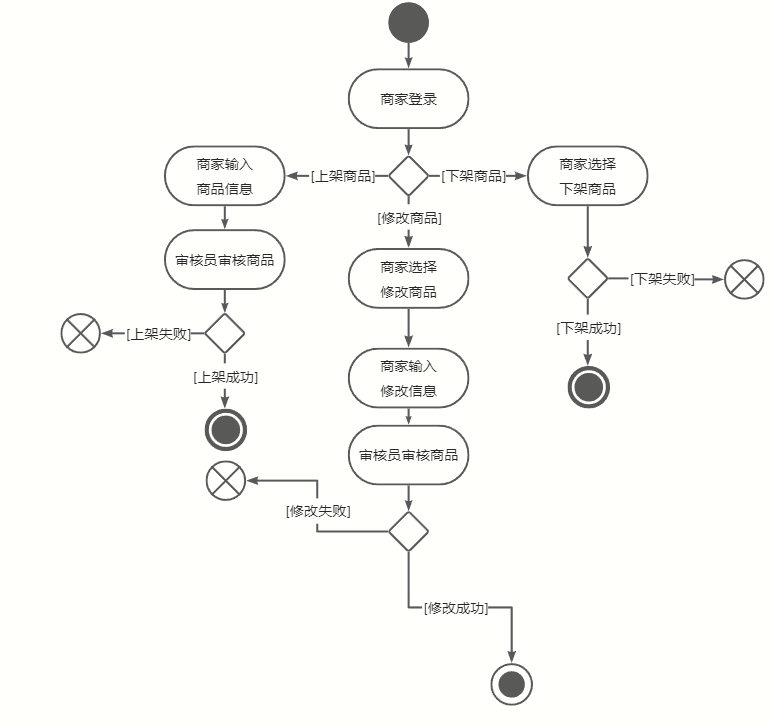
\includegraphics[width=0.6\linewidth]{pics/7.png}
    \caption{商家管理商品流程}
    \label{fig:sjglsplc}
\end{figure}

\section{功能性需求}
\subsection{执行者分析}
\begin{figure}[H]
    \centering
    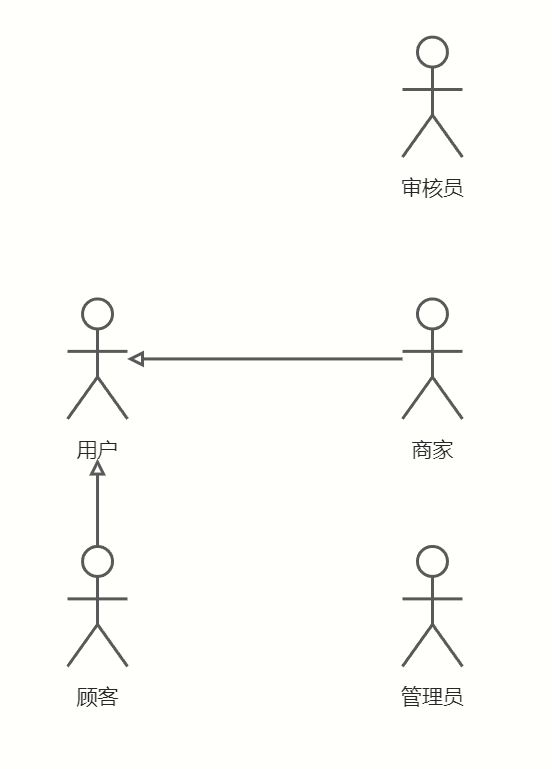
\includegraphics[width=0.4\linewidth]{pics/8.png}
    \caption{执行者分析}
    \label{fig:zxzfx}
\end{figure}

\subsection{总用例图}
\begin{figure}[H]
    \centering
    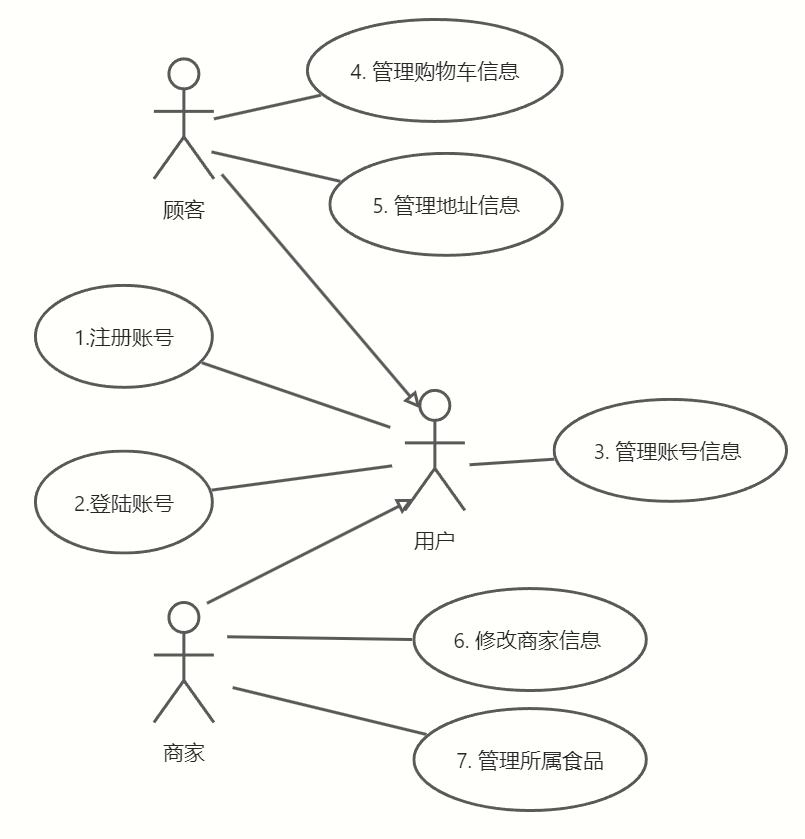
\includegraphics[width=0.75\linewidth]{pics/9.png}
    \caption{总用例图}
    \label{fig:zylt}
\end{figure}

\subsection{用户的用例}
\begin{figure}[H]
    \centering
    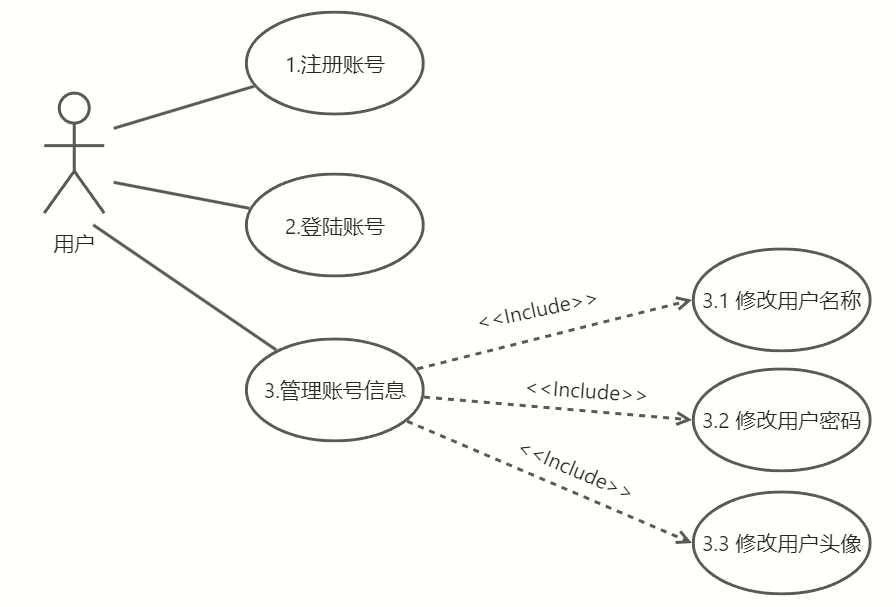
\includegraphics[width=0.75\linewidth]{pics/10.png}
    \caption{用户的用例}
    \label{fig:yhdyl}
\end{figure}


\begin{table}[h]
\resizebox{0.85\columnwidth}{!}{%
\begin{tabular}{|l|lll|}
\hline
编号   & \multicolumn{1}{l|}{1}    & \multicolumn{1}{l|}{名称}  & 注册账户 \\ \hline
执行者  & \multicolumn{1}{l|}{普通用户} & \multicolumn{1}{l|}{优先级} & 高    \\ \hline
描述   & \multicolumn{3}{l|}{用户使用手机号进行账户注册,设置账户密码}                   \\ \hline
前置条件 & \multicolumn{3}{l|}{输入正确的手机号码}                              \\ \hline
基本流程 & \multicolumn{3}{l|}{\begin{tabular}[c]{@{}l@{}}1.输入手机号码\\ 2.输入密码\\ 3.显示注册成功信息\end{tabular}}           \\ \hline
结束状况 & \multicolumn{3}{l|}{注册成功进入登录界面}                             \\ \hline
可选流程 & \multicolumn{3}{l|}{}                                       \\ \hline
异常流程 & \multicolumn{3}{l|}{\begin{tabular}[c]{@{}l@{}}1.手机号验证不通过,要求重新填写手机号\\ 2.用户已经注册显示用户已存在信息\end{tabular}} \\ \hline
描述   & \multicolumn{3}{l|}{}                                       \\ \hline
\end{tabular}%
}
\caption{}
\label{tab:1}
\end{table}


\begin{table}[H]
\resizebox{0.85\columnwidth}{!}{%
\begin{tabular}{|l|lll|}
\hline
编号   & \multicolumn{1}{l|}{2}                 & \multicolumn{1}{l|}{名称}             & 登录账户           \\ \hline
执行者  & \multicolumn{1}{l|}{普通用户}              & \multicolumn{1}{l|}{优先级}            & 高              \\ \hline
描述   & \multicolumn{3}{l|}{用户使用手机号进行账户登录}                                                            \\ \hline
前置条件 & \multicolumn{3}{l|}{\begin{tabular}[c]{@{}l@{}}1.提交正确的手机号码\\ 2.提交正确的密码\end{tabular}}          \\ \hline
基本流程 & \multicolumn{3}{l|}{\begin{tabular}[c]{@{}l@{}}1.输入手机号码\\ 2.输入密码\\ 3.显示登录成功信息\end{tabular}}   \\ \hline
结束状况 & \multicolumn{3}{l|}{\begin{tabular}[c]{@{}l@{}}1.登录成功进入主界面(注册时)\\ 2.登陆成功返回上一个页面\end{tabular}} \\ \hline
可选流程 & \multicolumn{3}{l|}{注册账号}                                                                     \\ \hline
异常流程 & \multicolumn{3}{l|}{\begin{tabular}[c]{@{}l@{}}1.手机号验证不通过,要求重新填写手机号\\ 2.用户未注册进入用户注册流程\\ 3.密码验证不通过\end{tabular}} \\ \hline
描述   & \multicolumn{3}{l|}{}                                                                         \\ \hline
\end{tabular}%
}
\caption{}
\label{tab:2}
\end{table}


\begin{table}[H]
\resizebox{0.85\columnwidth}{!}{%
\begin{tabular}{|l|lll|}
\hline
编号   & \multicolumn{1}{l|}{3.1}  & \multicolumn{1}{l|}{名称}  & 修改用户名称 \\ \hline
执行者  & \multicolumn{1}{l|}{普通用户} & \multicolumn{1}{l|}{优先级} & 低      \\ \hline
描述   & \multicolumn{3}{l|}{用户修改个人信息中的名称}                             \\ \hline
前置条件 & \multicolumn{3}{l|}{无}                                        \\ \hline
基本流程 & \multicolumn{3}{l|}{\begin{tabular}[c]{@{}l@{}}1.输入新用户名\\ 2.判断是否满足要求\\ 3.显示修改成功界面\end{tabular}}        \\ \hline
结束状况 & \multicolumn{3}{l|}{用户界面显示修改后的用户名}                            \\ \hline
可选流程 & \multicolumn{3}{l|}{\begin{tabular}[c]{@{}l@{}}1.用户名称不符合要求,重新输入\\ 2.用户名称已经存在,显示用户名称已经被使用\end{tabular}} \\ \hline
异常流程 & \multicolumn{3}{l|}{}                                         \\ \hline
描述   & \multicolumn{3}{l|}{}                                         \\ \hline
\end{tabular}%
}
\caption{}
\label{tab:3.1}
\end{table}

\begin{table}[H]
\resizebox{0.85\columnwidth}{!}{%
\begin{tabular}{|l|lll|}
\hline
编号   & \multicolumn{1}{l|}{3.2}  & \multicolumn{1}{l|}{名称}  & 修改用户密码 \\ \hline
执行者  & \multicolumn{1}{l|}{普通用户} & \multicolumn{1}{l|}{优先级} & 低      \\ \hline
描述   & \multicolumn{3}{l|}{用户修改个人信息中的密码}                             \\ \hline
前置条件 & \multicolumn{3}{l|}{1.旧密码输入正确}                                \\ \hline
基本流程 & \multicolumn{3}{l|}{\begin{tabular}[c]{@{}l@{}}1.输入新密码并再次输入确保无误\\ 2.判断是否满足密码要求\\ 3.显示密码修改成功界面\end{tabular}} \\ \hline
结束状况 & \multicolumn{3}{l|}{用户退出登录,需要重新输入新密码}                         \\ \hline
可选流程 & \multicolumn{3}{l|}{1.用户密码不符合要求,要求重新输入}                       \\ \hline
异常流程 & \multicolumn{3}{l|}{}                                         \\ \hline
描述   & \multicolumn{3}{l|}{}                                         \\ \hline
\end{tabular}%
}
\caption{}
\label{tab:3.2}
\end{table}

\begin{table}[H]
\resizebox{0.85\columnwidth}{!}{%
\begin{tabular}{|l|lll|}
\hline
编号   & \multicolumn{1}{l|}{3.3}  & \multicolumn{1}{l|}{名称}  & 修改用户头像 \\ \hline
执行者  & \multicolumn{1}{l|}{普通用户} & \multicolumn{1}{l|}{优先级} & 低      \\ \hline
描述   & \multicolumn{3}{l|}{用户修改个人信息中的头像}                             \\ \hline
前置条件 & \multicolumn{3}{l|}{}                                         \\ \hline
基本流程 & \multicolumn{3}{l|}{\begin{tabular}[c]{@{}l@{}}1.导入新头像\\ 2.判断是否满足大小要求\\ 3.显示头像修改成功界面\end{tabular}} \\ \hline
结束状况 & \multicolumn{3}{l|}{用户界面显示新头像}                                \\ \hline
可选流程 & \multicolumn{3}{l|}{1.图片大小不符合要求,要求重新导入}                       \\ \hline
异常流程 & \multicolumn{3}{l|}{}                                         \\ \hline
描述   & \multicolumn{3}{l|}{}                                         \\ \hline
\end{tabular}%
}
\caption{}
\label{tab:3.3}
\end{table}

\subsection{顾客的用例}
\begin{figure}[H]
    \centering
    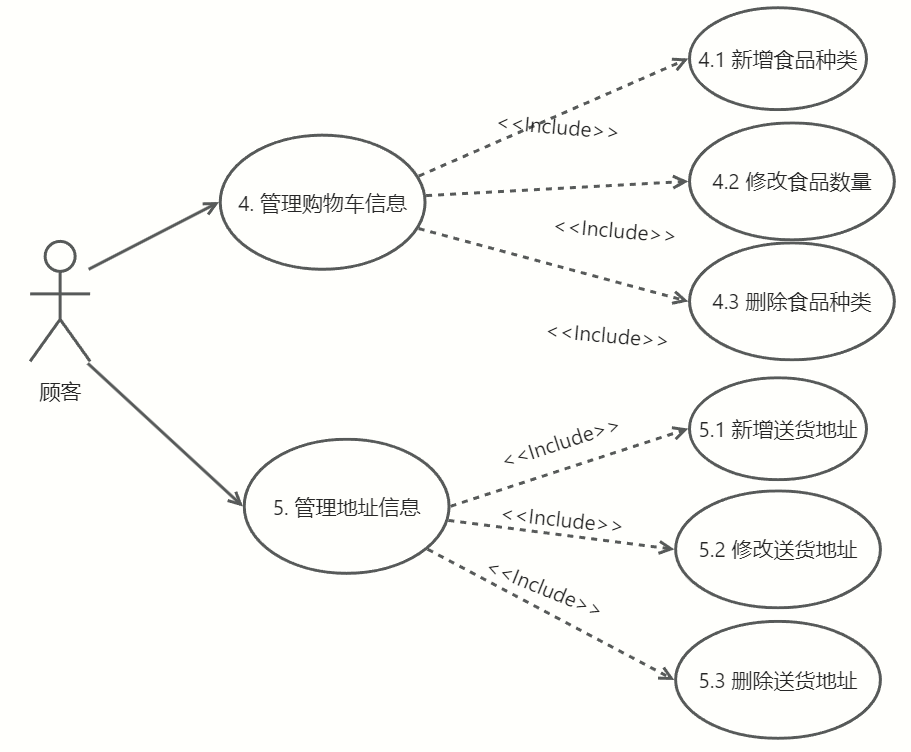
\includegraphics[width=0.8\linewidth]{pics/11.png}
    \caption{顾客的用例}
    \label{fig:gkdyl}
\end{figure}

\begin{table}[h]
\resizebox{0.85\columnwidth}{!}{%
\begin{tabular}{|l|lll|}
\hline
编号   & \multicolumn{1}{l|}{4}  & \multicolumn{1}{l|}{名称}  & 管理购物车信息 \\ \hline
执行者  & \multicolumn{1}{l|}{顾客} & \multicolumn{1}{l|}{优先级} & 低       \\ \hline
描述   & \multicolumn{3}{l|}{用户对购物车中商品进行新增,修改,删除操作}                   \\ \hline
前置条件 & \multicolumn{3}{l|}{登录用户}                                    \\ \hline
基本流程 & \multicolumn{3}{l|}{\begin{tabular}[c]{@{}l@{}}1.向购物车中添加商品\\ 2.修改商品的数量\\ 3.统计购物车内商品的总价格\end{tabular}} \\ \hline
结束状况 & \multicolumn{3}{l|}{\begin{tabular}[c]{@{}l@{}}得到一个完整的购物车内容\\ 超过起送费即可生成订单\end{tabular}}               \\ \hline
可选流程 & \multicolumn{3}{l|}{1.删除购物车中的商品.}                            \\ \hline
异常流程 & \multicolumn{3}{l|}{}                                        \\ \hline
描述   & \multicolumn{3}{l|}{}                                        \\ \hline
\end{tabular}%
}
\caption{}
\label{tab:4}
\end{table}

\begin{table}[H]
\resizebox{0.85\columnwidth}{!}{%
\begin{tabular}{|l|lll|}
\hline
编号   & \multicolumn{1}{l|}{5.1} & \multicolumn{1}{l|}{名称}  & 新增送货地址 \\ \hline
执行者  & \multicolumn{1}{l|}{顾客}  & \multicolumn{1}{l|}{优先级} & 低      \\ \hline
描述   & \multicolumn{3}{l|}{顾客新增地址列表中的送货地址}                          \\ \hline
前置条件 & \multicolumn{3}{l|}{}                                        \\ \hline
基本流程 & \multicolumn{3}{l|}{\begin{tabular}[c]{@{}l@{}}1.点击地址界面的新建用户地址\\ 2.依次填入地址信息满足正常地址规范\\ 3.显示新建地址成功界面\end{tabular}} \\ \hline
结束状况 & \multicolumn{3}{l|}{用户界面出现新地址的简略版本}                          \\ \hline
可选流程 & \multicolumn{3}{l|}{\begin{tabular}[c]{@{}l@{}}1.用户输入的地址不符合正常的地址规范,需要重新输入\\ 2.地址中的必填信息未填写,需要写入\end{tabular}}     \\ \hline
异常流程 & \multicolumn{3}{l|}{}                                        \\ \hline
描述   & \multicolumn{3}{l|}{}                                        \\ \hline
\end{tabular}%
}
\caption{}
\label{tab:5.1}
\end{table}

\begin{table}[H]
\resizebox{0.85\columnwidth}{!}{%
\begin{tabular}{|l|lll|}
\hline
编号   & \multicolumn{1}{l|}{5.2}                 & \multicolumn{1}{l|}{名称}                  & 修改送货地址                 \\ \hline
执行者  & \multicolumn{1}{l|}{顾客}                  & \multicolumn{1}{l|}{优先级}                 & 低                      \\ \hline
描述   & \multicolumn{3}{l|}{顾客修改地址列表中的送货地址}                                                                          \\ \hline
前置条件 & \multicolumn{3}{l|}{}                                                                                        \\ \hline
基本流程 & \multicolumn{3}{l|}{\begin{tabular}[c]{@{}l@{}}1.点击地址界面的用户地址\\ 2.修改地址信息满足正常地址规范\\ 3.显示修改地址成功界面\end{tabular}} \\ \hline
结束状况 & \multicolumn{3}{l|}{用户界面出现修改后的新地址的简略版本}                                                                      \\ \hline
可选流程 & \multicolumn{3}{l|}{\begin{tabular}[c]{@{}l@{}}1.用户输入的地址不符合正常的地址规范,需要重新输入\\ 2.地址中的必填信息未填写,需要写入\end{tabular}} \\ \hline
异常流程 & \multicolumn{3}{l|}{}                                                                                        \\ \hline
描述   & \multicolumn{3}{l|}{}                                                                                        \\ \hline
\end{tabular}%
}
\caption{}
\label{tab:5.2}
\end{table}

\begin{table}[H]
\resizebox{0.85\columnwidth}{!}{%
\begin{tabular}{|l|lll|}
\hline
编号   & \multicolumn{1}{l|}{5.3} & \multicolumn{1}{l|}{名称}  & 删除送货地址 \\ \hline
执行者  & \multicolumn{1}{l|}{顾客}  & \multicolumn{1}{l|}{优先级} & 低      \\ \hline
描述   & \multicolumn{3}{l|}{顾客删除地址列表中的送货地址}                          \\ \hline
前置条件 & \multicolumn{3}{l|}{1.地址列表中有已经存在的地址}                         \\ \hline
基本流程 & \multicolumn{3}{l|}{\begin{tabular}[c]{@{}l@{}}1.点击地址界面的用户地址,进入用户的地址列表界面\\ 2.选中需要删除的地址,点击删除,询问是否删除\\ 3.显示删除地址成功界面\end{tabular}} \\ \hline
结束状况 & \multicolumn{3}{l|}{用户的地址列表界面原地址消失}                          \\ \hline
可选流程 & \multicolumn{3}{l|}{1.误触点到删除,询问是否删除时点击否,返回用户地址列表界面}          \\ \hline
异常流程 & \multicolumn{3}{l|}{}                                        \\ \hline
描述   & \multicolumn{3}{l|}{}                                        \\ \hline
\end{tabular}%
}
\caption{}
\label{tab:5.3}
\end{table}

\subsection{商家的用例}
\begin{figure}[H]
    \centering
    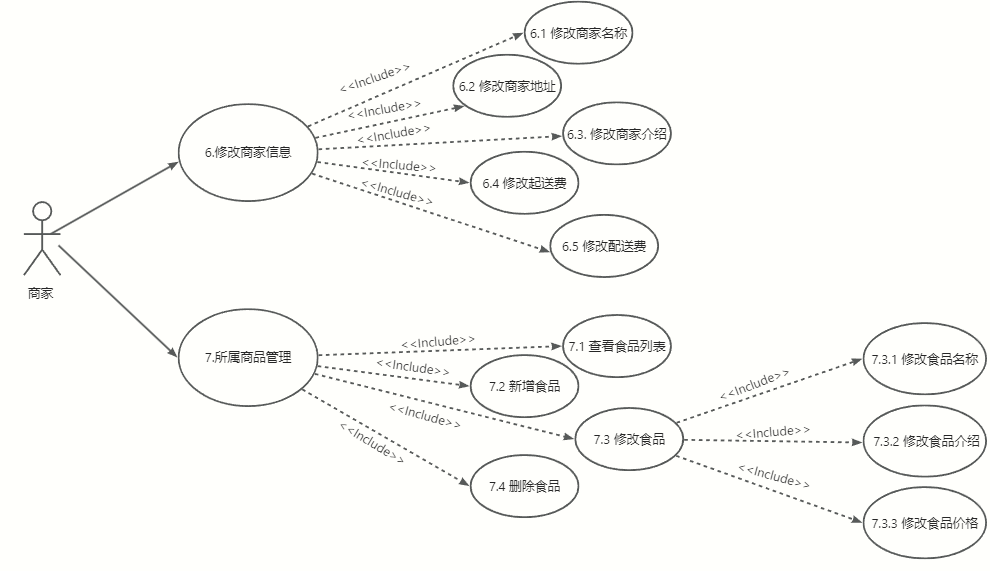
\includegraphics[width=1\linewidth]{pics/12.png}
    \caption{商家的用例}
    \label{fig:sjdyl}
\end{figure}

\begin{table}[H]
\resizebox{0.85\columnwidth}{!}{%
\begin{tabular}{|l|lll|}
\hline
编号   & \multicolumn{1}{l|}{6.1} & \multicolumn{1}{l|}{名称}  & 修改商家名称 \\ \hline
执行者  & \multicolumn{1}{l|}{商家}  & \multicolumn{1}{l|}{优先级} & 低      \\ \hline
描述   & \multicolumn{3}{l|}{商家修改商家信息中的名称}                            \\ \hline
前置条件 & \multicolumn{3}{l|}{无}                                       \\ \hline
基本流程 & \multicolumn{3}{l|}{\begin{tabular}[c]{@{}l@{}}1.输入新商家名\\ 2.判断是否满足要求\\ 3.显示修改成功界面\end{tabular}}        \\ \hline
结束状况 & \multicolumn{3}{l|}{商家界面显示修改后的商家名}                           \\ \hline
可选流程 & \multicolumn{3}{l|}{\begin{tabular}[c]{@{}l@{}}1.用户名称不符合要求,重新输入\\ 2.用户名称已经存在,显示用户名称已经被使用\end{tabular}} \\ \hline
异常流程 & \multicolumn{3}{l|}{}                                        \\ \hline
描述   & \multicolumn{3}{l|}{}                                        \\ \hline
\end{tabular}%
}
\caption{}
\label{tab:6.1}
\end{table}

\begin{table}[H]
\resizebox{0.85\columnwidth}{!}{%
\begin{tabular}{|l|lll|}
\hline
编号   & \multicolumn{1}{l|}{6.2} & \multicolumn{1}{l|}{名称}  & 修改商家地址 \\ \hline
执行者  & \multicolumn{1}{l|}{商家}  & \multicolumn{1}{l|}{优先级} & 低      \\ \hline
描述   & \multicolumn{3}{l|}{商家修改商家信息中的地址}                            \\ \hline
前置条件 & \multicolumn{3}{l|}{无}                                       \\ \hline
基本流程 & \multicolumn{3}{l|}{\begin{tabular}[c]{@{}l@{}}1.输入商家的新地址\\ 2.判断是否满足正常的地址规范\\ 3.显示地址修改成功界面\end{tabular}} \\ \hline
结束状况 & \multicolumn{3}{l|}{商家界面显示修改后的商家地址}                          \\ \hline
可选流程 & \multicolumn{3}{l|}{1.商家地址不符合要求,重新输入}                        \\ \hline
异常流程 & \multicolumn{3}{l|}{}                                        \\ \hline
描述   & \multicolumn{3}{l|}{}                                        \\ \hline
\end{tabular}%
}
\caption{}
\label{tab:6.2}
\end{table}

\begin{table}[H]
\resizebox{0.85\columnwidth}{!}{%
\begin{tabular}{|l|lll|}
\hline
编号   & \multicolumn{1}{l|}{6.3} & \multicolumn{1}{l|}{名称}  & 修改商家介绍 \\ \hline
执行者  & \multicolumn{1}{l|}{商家}  & \multicolumn{1}{l|}{优先级} & 低      \\ \hline
描述   & \multicolumn{3}{l|}{商家修改商家信息中的介绍}                            \\ \hline
前置条件 & \multicolumn{3}{l|}{无}                                       \\ \hline
基本流程 & \multicolumn{3}{l|}{\begin{tabular}[c]{@{}l@{}}1.输入商家的新介绍\\ 2.判断是否满足要求(字数要求,敏感词)\\ 3.显示修改成功界面\end{tabular}} \\ \hline
结束状况 & \multicolumn{3}{l|}{商家界面显示修改后的商家介绍}                          \\ \hline
可选流程 & \multicolumn{3}{l|}{1.商家介绍不符合要求,重新输入}                        \\ \hline
异常流程 & \multicolumn{3}{l|}{}                                        \\ \hline
描述   & \multicolumn{3}{l|}{}                                        \\ \hline
\end{tabular}%
}
\caption{}
\label{tab:6.3}
\end{table}

\begin{table}[H]
\resizebox{0.85\columnwidth}{!}{%
\begin{tabular}{|l|lll|}
\hline
编号   & \multicolumn{1}{l|}{6.4} & \multicolumn{1}{l|}{名称}  & 修改商家起送费 \\ \hline
执行者  & \multicolumn{1}{l|}{商家}  & \multicolumn{1}{l|}{优先级} & 低       \\ \hline
描述   & \multicolumn{3}{l|}{商家修改商家信息中的起送费}                            \\ \hline
前置条件 & \multicolumn{3}{l|}{无}                                        \\ \hline
基本流程 & \multicolumn{3}{l|}{\begin{tabular}[c]{@{}l@{}}1.输入商家的新起送费\\ 2.判断是否满足要求(选择:免起送费,固定金额)\\ 3.显示修改成功界面\end{tabular}} \\ \hline
结束状况 & \multicolumn{3}{l|}{\begin{tabular}[c]{@{}l@{}}商家下单界面显示修改后的新起送费\\ 只要满足订单金额大于起送费时,订单才允许跳转到支付界面\end{tabular}}      \\ \hline
可选流程 & \multicolumn{3}{l|}{1.商家起送费不符合要求,重新输入}                        \\ \hline
异常流程 & \multicolumn{3}{l|}{}                                         \\ \hline
描述   & \multicolumn{3}{l|}{}                                         \\ \hline
\end{tabular}%
}
\caption{}
\label{tab:6.4}
\end{table}

\begin{table}[H]
\resizebox{0.85\columnwidth}{!}{%
\begin{tabular}{|l|lll|}
\hline
编号   & \multicolumn{1}{l|}{6.5} & \multicolumn{1}{l|}{名称}  & 修改商家配送费 \\ \hline
执行者  & \multicolumn{1}{l|}{商家}  & \multicolumn{1}{l|}{优先级} & 低       \\ \hline
描述   & \multicolumn{3}{l|}{商家修改商家信息中的配送费}                            \\ \hline
前置条件 & \multicolumn{3}{l|}{无}                                        \\ \hline
基本流程 & \multicolumn{3}{l|}{\begin{tabular}[c]{@{}l@{}}1.输入商家新的配送费\\ 2.判断是否满足要求(金额要求)\\ 3.显示修改成功界面\end{tabular}} \\ \hline
结束状况 & \multicolumn{3}{l|}{商家下单界面显示修改后的配送费}                          \\ \hline
可选流程 & \multicolumn{3}{l|}{1.商家配送费不符合要求,重新输入}                        \\ \hline
异常流程 & \multicolumn{3}{l|}{}                                         \\ \hline
描述   & \multicolumn{3}{l|}{}                                         \\ \hline
\end{tabular}%
}
\caption{}
\label{tab:6.5}
\end{table}

\subsection{其他功能性需求}
在"我的"页面通过"成为商家"功能对用户权限进行修改,成为商家之后在"我的"页面会显示"店铺管理"功能,进入"店铺管理"功能页面即可执行商家相关功能.

\section{非功能性需求}
\subsection{系统架构要求}

\begin{figure}[H]
    \centering
    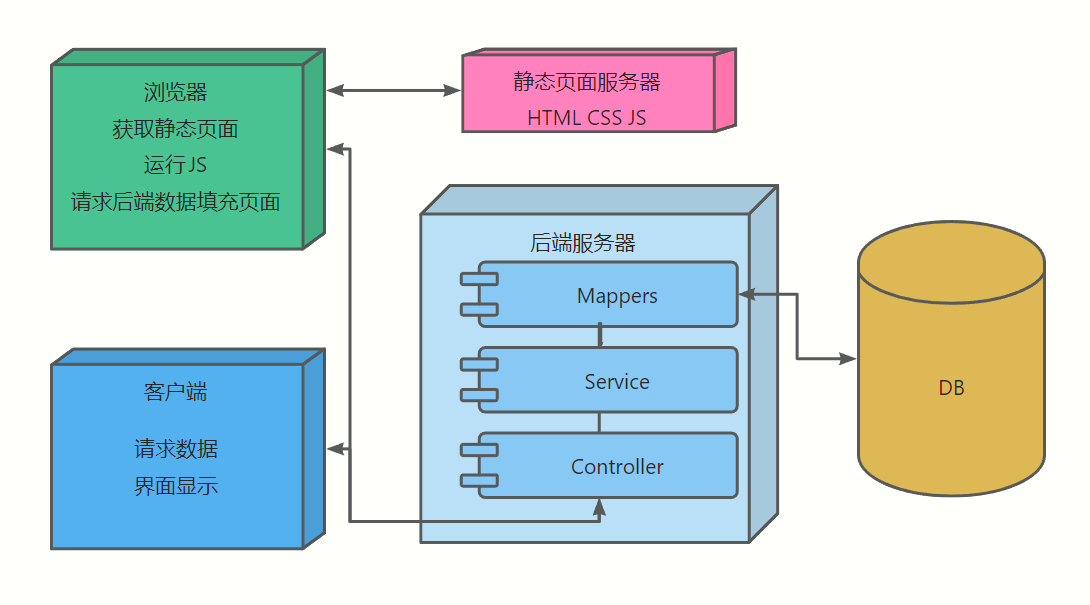
\includegraphics[width=1\linewidth]{pics/13.png}
    \caption{系统架构}
    \label{fig:xtjj}
\end{figure}
\subsubsection{微服务架构}
服务拆分:饿了吧的业务逻辑复杂,包括用户管理、商户管理、订单处理、支付系统等多个模块。微服务架构将这些模块拆分为独立的服务,便于各自独立开发、部署和维护。不仅提高了开发效率,还增强了系统的可扩展性和容错能力。


\subsection{接口API}
\subsubsection*{business}
\begin{itemize}
    \item \textbf{ businesses/orderType/{orderTypeId}}
    \begin{itemize}
    \item 请求方法:GET
    \item 参数:orderTypeId
    \item 返回值:business 数组
    \item 功能:根据点餐分类编号查询分类商家信息
    \item 后端函数名:listBusinessByOrderTypeId
    \end{itemize}
    \item businesses/{businessId}
    \begin{itemize}
    \item 请求方法:GET
    \item 参数:businessId
    \item 返回值:businessId对象
    \item 功能:根据商家编号查询商家信息
    \item 后端函数名:getBusinessById
    \end{itemize}
    \item businesses
    \begin{itemize}
    \item 请求方法:POST
    \item 参数:businessName、businessImg、orderTypeId
    \item 返回值:int(返回行数)
    \item 功能:向商家表中添加一条字段
    \item 后端函数名:r egisterBusiness
    \end{itemize}
    \item businesses
    \begin{itemize}
    \item 请求方法:PUT
    \item 参数:businessId、businessName、businessAddress、businessExplain、businessImg、orderTypeId、starPrice、deliveryPrice
    \item 返回值:int(返回影响的行数)
    \item 功能:向商家表中更新一条记录
    \item 后端函数名:updateBusiness
    \end{itemize}
    \item 5. businesses
    \begin{itemize}
    \item 请求方法:DELETE
    \item 参数:businessId
    \item 返回值:int(删除成功)
    \item 功能:根据商家编号删除一条商家记录(将delTag设为0)
    \item 后端函数名:deleteBusiness
    \end{itemize}
\end{itemize}

\subsubsection*{food}
\begin{itemize}
   
    \item foods/business/{businessId}
     \begin{itemize}
    \item 请求方法:GET
    \item 参数:businessId
    \item 返回值:food 数组
    \item 功能:根据商家编号查询所属食品信息
    \item 后端函数名:listFoodByBusinessId
    \end{itemize}
    \item foods/{foodId}
    \begin{itemize} 
    \item 请求方法:GET
    \item 参数:foodId
    \item 返回值:food对象
    \item 功能:根据食品编号查询食品信息
    \item 后端函数名:getFoodById
    \end{itemize}
    \item foods
    \begin{itemize}
    \item 请求方法:POST
    \item 参数:foodName、foodExplain、foodImg、foodPrice、businessId、quantity
    \item 返回值:int
    \item 功能:向食品表中添加一条记录
    \item 后端函数名:addfood
    \end{itemize}
    \item foods/{foodId}
    \begin{itemize}
    \item 请求方法:PUT
    \item 参数:businessId、foodId、foodName、foodExplain、foodImg、foodPrice、quantity
    \item 返回值:int
    \item 功能:根据商家编号、食品编号更新一条食品记录(检测商家是否匹配,更新前拷贝)
    \item 后端函数名:updateFood
    \end{itemize}
    \item foods
    \begin{itemize}
    \item 请求方法:PATCH
    \item 参数:businessId、foodId、soldOut
    \item 返回值:int
    \item 功能:根据商家编号、食品编号更新食品是否售罄
    \item 后端函数名:setFood
   \end{itemize}
    \item foods/{foodId}
    \begin{itemize}
    \item 请求方法:DELETE
    \item 参数:businessId、foodId
    \item 返回值:int
    \item 功能:根据商家编号、食品编号删除一条食品记录(将delTag设为0,检测商家是否匹配,删除前拷贝)
    \item 后端函数名:removeFood
    \end{itemize}
\end{itemize}


\subsubsection*{cart}
\begin{itemize}
    \item  carts/user/{userId}/{businessId}
    \begin{itemize}
    \item 请求方法:GET
    \item 参数:userId、businessId(可选)
    \item 返回值:cart数组(多对一:所属商家信息、所属食品信息)
    \item 功能:据用户编号和商家编号,查询此用户购物车中某个商家的所有购物车信息
    \item 后端函数名:listCart
    \end{itemize}
    \item carts
    \begin{itemize}
    \item 请求方法:POST
    \item 参数:userId、businessId、foodId
    \item 返回值:int
    \item 功能:向购物车表中添加一条记录
    \item 后端函数名:saveCart
    \end{itemize}
    \item  carts
    \begin{itemize}
    \item 请求方法:PUT
    \item 参数:userId、businessId、foodId、quantity
    \item 返回值:int
    \item 功能:根据用户编号、商家编号、食品编号更新数量
    \item 后端函数名:updateCart
    \end{itemize}
    \item carts
    \begin{itemize}
    \item 请求方法:DELETE
    \item 参数:userId、businessId、foodId(可选)
    \item 返回值:int
    \item 功能:根据用户编号、商家编号、食品编号删除购物车表中的一条食品记录
    \item 根据用户编号、商家编号删除购物车表中的多条记录
    \item 后端函数名:removeCart
    \end{itemize}
\end{itemize}

\subsubsection*{deliveryAddress}
\begin{itemize}
\item delivery-addresses/user/{userId}
\begin{itemize}
    \item 请求方法:GET
    \item 参数:userId
    \item 返回值:deliveryAddress数组
    \item 功能:根据用户编号查询所属送货地址
    \item 后端函数名:listDeliveryAddressByUserId
\end{itemize}

\item delivery-addresses/{daId}
\begin{itemize}
    \item 请求方法:GET
    \item 参数:daId
    \item 返回值:deliveryAddress对象
    \item 功能:根据送货地址编号查询送货地址
    \item 后端函数名:getDeliveryAddressById
\end{itemize}

\item delivery-addresses
\begin{itemize}
    \item 请求方法:POST
    \item 参数:contactName、contactSex、contactTel、address、userId
    \item 返回值:int
    \item 功能:向送货地址表中添加一条记录
    \item 后端函数名:saveDeliveryAddress
\end{itemize}

\item delivery-addresses
\begin{itemize}
    \item 请求方法:PUT
    \item 参数:daId、contactName、contactSex、contactTel、address、userId
    \item 返回值:int
    \item 功能:根据送货地址编号更新送货地址信息(更新前拷贝)
    \item 后端函数名:updateDeliveryAddress
\end{itemize}

\item delivery-addresses/{daId}
\begin{itemize}
    \item 请求方法:DELETE
    \item 参数:daId
    \item 返回值:int
    \item 功能:根据送货地址编号删除一条记录(删除前拷贝)
    \item 后端函数名:removeDeliveryAddress
\end{itemize}
\end{itemize}

\subsubsection*{order}
\begin{itemize}
\item orders/user/{userId}
\begin{itemize}
    \item 请求方法:GET
    \item 参数:userId
    \item 返回值:orders数组(包括多对一:business; 一对多:订单明细信息)
    \item 功能:根据用户编号查询此用户的所有订单信息
    \item 后端函数名:listOrdersByUserId
\end{itemize}

\item orders/{orderId}
\begin{itemize}
    \item 请求方法:GET
    \item 参数:userId
    \item 返回值:orders数组(包括多对一:business; 一对多:订单明细信息)
    \item 功能:根据订单编号查询订单信息,包括所属商家信息,和此订单的所有订单明细信息
    \item 后端函数名:getOrdersById
\end{itemize}

\item orders
\begin{itemize}
    \item 请求方法:POST
    \item 参数:userId、businessId、daId、orderTotal
    \item 返回值:int
    \item 功能:\par
        1. 用户编号、商家编号、订单总金额、送货地址编号向订单表中添加一条记录,并获取自动生成的订单编号\par
         2. 根据用户编号、商家编号从购物车表中查询所有数据,批量添加到订单明细表中\par
        3. 根据用户编号、商家编号删除购物车表中的数据。
    \item 后端函数名:createOrders
\end{itemize}
\end{itemize}

\subsubsection*{user}
\begin{itemize}
\item users/login
\begin{itemize}
    \item 请求方法:POST
    \item 参数:userId、password
    \item 返回值:user对象
    \item 功能:根据用户编号与密码查询用户信息
    \item 后端函数名:getUserByIdByPass
\end{itemize}

\item users/{userId}
\begin{itemize}
    \item 请求方法:GET
    \item 参数:userId
    \item 返回值:int
    \item 功能:根据用户编号查询用户表返回的行数
    \item 后端函数名:getUserById
\end{itemize}

\item users/register
\begin{itemize}
    \item 请求方法:POST
    \item 参数:userId、password、userName、userSex
    \item 返回值:int
    \item 功能:向用户表中添加一条记录
    \item 后端函数名:saveUser
\end{itemize}

\item users
\begin{itemize}
    \item 请求方法:PUT
    \item 参数:userId、password、userName、userSex、userImg(可选)
    \item 返回值:int
    \item 功能:根据用户编号与密码更改用户信息
    \item 后端函数名:updateUser
\end{itemize}

\item users
\begin{itemize}
    \item 请求方法:DELETE
    \item 参数:userId、password
    \item 返回值:int
    \item 功能:根据用户编号与密码删除用户(将delTag设为0)
    \item 后端函数名:deleteUser
\end{itemize}
\end{itemize}
\subsubsection*{key}
\begin{itemize}
  \item public-key
\begin{itemize}
    \item 请求方法:GET
    \item 参数:
    \item 返回值:string
    \item 功能:根据后端的私钥生成公钥返回到前端
    \item 后端函数名:getPublicKey
\end{itemize}
\end{itemize}

\subsubsection*{captcha}
\begin{itemize}
 \item captcha
\begin{itemize}
    \item 请求方法:GET
    \item 参数:session
    \item 返回值:byte[]
    \item 功能:生成验证码图片发送到前端
    \item 后端函数名:getCaptcha
\end{itemize}

 \item captcha

\begin{itemize}
    \item 请求方法:POST
    \item 参数:session,captchaInput
    \item 返回值:ture or false
    \item 功能:对前端发来的验证码进行验证
    \item 后端函数名:verifyCaptcha
\end{itemize}
\end{itemize}


\subsection{安全性}
饿了吧在前后端采用多种方案共同实现对于用户敏感信息的保护:
\begin{itemize}
    \item 在传输密码时,使用HTTP POST进行传输,不在URL中传输敏感数据
    \item 实现登录时,对密码的传输首先在前端接收后端发送的公钥,在前端对密码进行加密,前端传到后端的内容为密文,密文在后端进行解密,保证传输过程的密码安全性
    \item 用户注册时,后端将会对密码进行哈希加密处理之后再存入数据库.保存在数据库中的密码为哈希值,有效防止数据库被入侵后导致用户密码信息的泄露风险
\end{itemize}


另外,我们在需要登录信息才能访问的页面发送的请求中附带token,在前端,我们在创建好的axios实例axiosInstance上,挂载两个拦截器:
\begin{itemize}
\item 请求拦截器:
\begin{itemize}
    \item 前端向后端发送请求之前拦截;
    \item 在header添加token,若有请求错误,在控制台打出
\end{itemize}
\item 响应拦截器:
\begin{itemize}
    \item 后端向前端发送响应,前端接到之后拦截;
    \item 处理响应状态码错误401,500等
    \item 网络错误,重试三次,重试失败,跳转回主页;
    \item 重试次数超过最大限制3,跳转回主页
\end{itemize}
\end{itemize}

后端接到请求后,进入controller层之前拦截;
登录成功后得到token并发回前端,后所有请求都需加上token;
被拦截的请求发回500错误码;
拦截涉及用户信息的请求,有关拦截过滤的内容在WebMvcConfig文件配置,需精细到请求方法的在TokenInterceptor配置;

同时,为了预防恶意脚本使用大量相同请求对于服务器的攻击,我们设计了验证码人机验证的接口,主要是在用户下订单流程中,同一订单中商品超过一定数量就会触发人机验证,通过从后端接收随机生成的,经过多重模糊化处理的多位数字图片进行人机验证,用户根据验证码图片的内容填写验证码,验证失败则拒绝改次对服务器的访问,从而保证了服务器的安全.




\subsection{性能}
无
\subsection{界面}
饿了吧的界面风格强调简洁、现代和用户友好,界面流的设计目的是让用户能够快速、顺畅地完成点餐和支付。首页设计则突出了搜索、分类导航、订单和用户信息管理,确保用户能够快速找到所需的内容。商家后台的报表功能详细且直观,帮助商家有效管理和分析经营数据,优化服务质量。
\subsubsection{界面风格}
在界面风格的设计上,饿了吧秉持简洁、现代、友好的设计思路,遵循以下几个特点:
\begin{itemize}
    \item 颜色搭配:主色调为蓝色和白色,蓝色作为品牌的标志性颜色,用于导航栏、按钮等高亮位置,白色背景确保信息清晰易读。辅助色(如橙色、红色)用作重要信息提示,增强视觉对比。
    \item 扁平化设计:饿了吧采用扁平化设计语言,图标简洁、信息模块化,整体界面更加简约和直观。
    \item 图标和插图:界面中使用卡通风格的图标和插图,增强了友好度.
    \item 响应式设计:饿了吧的设计能够适应各种设备屏幕,从手机到平板和电脑,界面元素会根据屏幕尺寸动态调整,保证了用户体验的一致性。
\end{itemize}

\subsubsection{界面流}
饿了吧的界面流设计注重用户体验的顺畅性和任务的高效完成,在页面路由的设计上力争以最高效的流程实现业务操作
\subsubsection{首页}
饿了吧的首页设计简洁直观,旨在让用户快速找到所需的餐厅或商品。
\subsubsection{报表信息}
饿了吧计划提供功能丰富的后台系统,方便商家查看订单数据、经营情况和各类分析报表。











\end{document}                                 % 结束全文
